\section{Classification}

Recall that the question we wish to explore in this thesis is whether training an autoencoder has benefits over models trained simply on labeled data. As a benchmark we trained a linear model on the data-representations from a pre-trained VGG16 network. This high-performing model from the image analysis community has seen successful applications to the same experimental data, and so is a reasonable comparison for our methods (\cite{Kuchera2019}). 

\subsection{Convolutional autoencoder}
Using the \lstinline{RandomSearch} framework we were able to find a network configuration for the convolutional autoencoder that shows very strong performance on the simulated data. And strong performance on the filtered and full datasets. From the hyper-parameter search listed in appendix \ref{appendix:hyperparams}\todo{add tables for searches with real and filtered} and the best models found, and listed in table \ref{tab:best_params_clf_convae}, we observe that there are no obvious relationships between most of the hyper-parameters and classification performance. The maximum-mean-discrepancy seems to trend with higher performance, as well as a fairly large first kernel. This result can be attributed to the performance landscape being very multi-modal with respect to the classification performance. Then there are many configurations that satisfy a linearly separable latent space. However there is also a large variation in the latent space indicating that there are regions of the hyper-parameter space that are unsuited to the purpose of making linearly separable latent spaces. \todo{Investigate with static random search - isolating some hyperparams} 

\subsubsection{Latent space}
Regarding the configuration of the latent space we note a preference for the maximum mean discrepancy term in terms of classifier performance. As \citet{Antoran2019} shows the mapping of the latent space to an isotropic Gaussian distribution as the Kullback-Leibler objective aims to achieve contributes to the washing out of class information, but strongly encourages feature information. \citet{Antoran2019} describes feature information as e.g stroke thickness or skew when drawing a number, while class information is the more esoteric "five"-ness of all drawings of the number five.

\begin{figure}
\centering
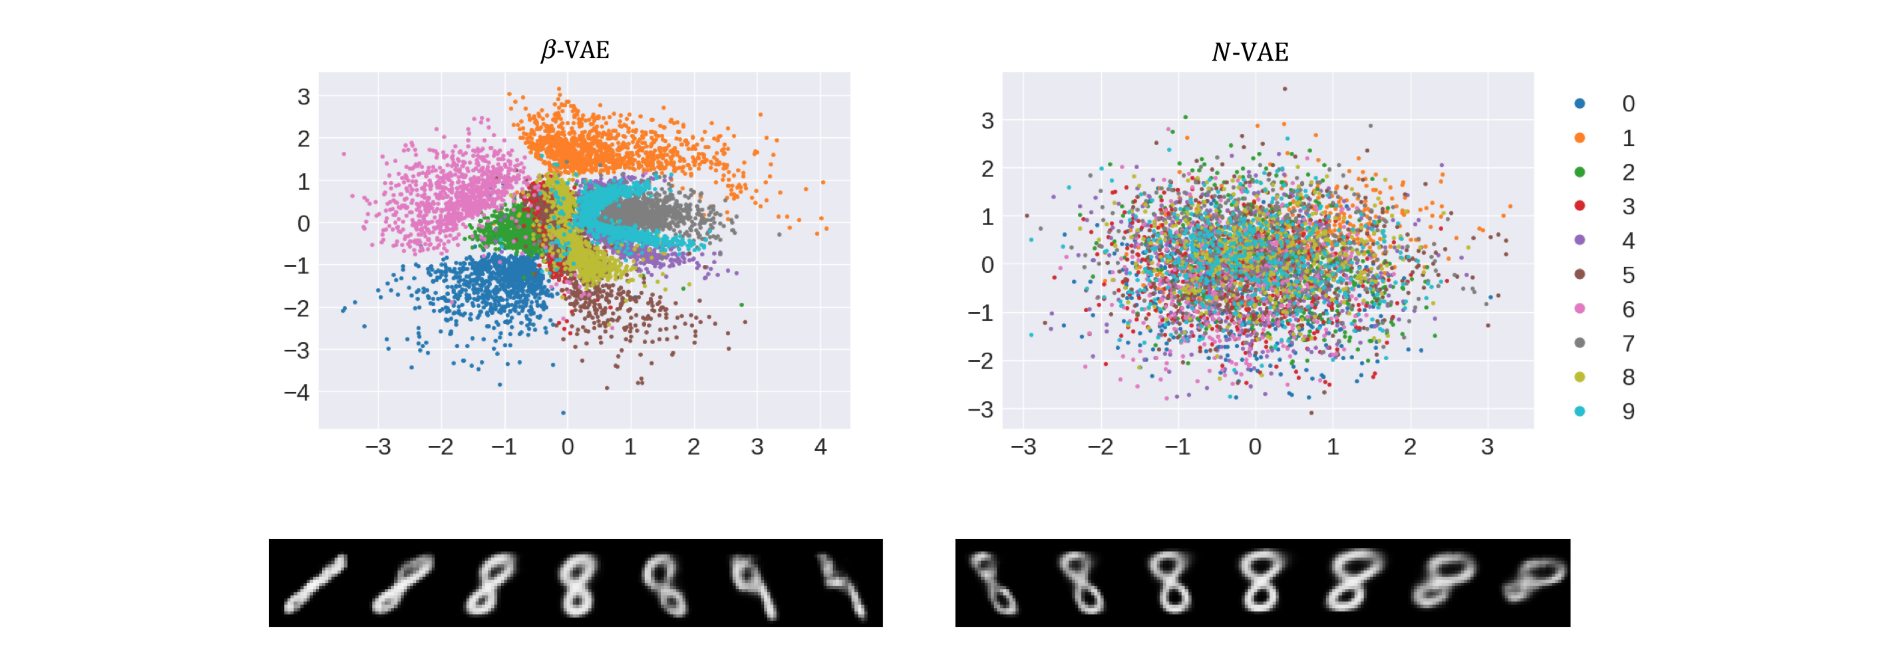
\includegraphics[width=\textwidth, height=3in]{plots/latent_traversal}
\caption[Difference between generative and discriminative latent spaces]{Demonstrating the difference of capturing class and feature information in the latent space. On the left the $\beta$-VAE pushes the autoencoder to a representation favoring encoded class information in the latent space. The spaces between the class blobs makes for a poor generative algorithm, but for the purpose of classification or even clustering this is strongly preferable. On the right the natural clustering of feature information is demonstrated by the convincingly isotropic nature of the latent space distribution. The subplots under the latent distributions demonstrate reconstructions of a traversal along a latent axis, clearly showing the difference between feature and class information. Figure copied from \citet{Antoran2019}}\label{fig:latent_traversal}
\end{figure}

Indeed this objective works in favor of the variational autoencoder by tightening the distribution, i.e. achieving a density in the latent space without holes, that allows for the generation of new samples without areas in the latent space that do not have a corresponding output. 

An additional challenge attached to the latent space is the problem that the decoder might have the capacity to be trained as an autodecoder, i.e. reconstructing almost independently from the latent sample\todo{add citations from DD-paper}. This problem is investigated in detail by \todo{add citation to DD paper} where they propose the dueling decoder structure. The dueling decoder adds a second reconstruction term to the objective. This second reconstruction is optimized over a different representation of the data. This might be reconstructing the edges in an image, it's intensity histogram or other transformations. For applications in physics this is a promising approach as it allows the inclusion of physical properties to the optimization. For the AT-TPC data this includes predicting the charge-intensity profile or the total charge deposited during the event.

\subsubsection{Classifier performance}

From table \ref{tab:clf_no_vgg} it's clear that while the autoencoder architecture, \ref{item:clf_no_vgg}, is able to capture class information it does not outperform the pre-trained VGG16 in terms of the linear separability of its latent space. Regarding the performance in terms of the number of latent samples there seems to be no indication that performance was increased in that regard either. Visually inspecting the latent space in figure \ref{fig:ac_tnse} we observe the same separation between proton and carbon events for simulated data. For the filtered and full datasets we observe a slight degradation of proton separation compared to the pure VGG16 representation, which we confirm by the proton $f1$ scores in table \ref{tab:clf_no_vgg}. Carbon is consistently hard to separate from the amorphous "other" category, and there is no indication that the autoencoder is able to separate them better than the pure VGG16 latent space is. 

Using the VGG16 representation as an initial encoded representation, \ref{item:clf_freeze_vgg} improved performance substantially from the \ref{item:clf_no_vgg} architecture. The mean performance is  close to the VGG16 performance, but the standard error is larger. \todo{do z tests of same mean I suppose?} Inspecting the performance as a function of  n-labeled samples we observe that the \ref{item:clf_freeze_vgg} autoencoder exhibits the same  patterns of error with almost zero deviation from the mean for the filtered and simulated data, but with variations in the second decimal for the full data. The same behavior is seen in the pure VGG16 classifiers performance.

The obvious question is then why the reconstruction objective does not aid in classification. To find a plausible answer we look to a discussion on the PCA from \cite{Jolliffe1982} where he remarks that the major axes of variation may not be the ones carrying class information. This relates to the reconstruction objective where we posit that the reconstruction focuses the optimization over these major axes of variation, and if they do not carry the salient class-separating information there is no reason to believe the latent space would. Adding to this argument is the observation that adding the dueling decoder improves the classifier. The representations chosen for the auxiliary optimization task are salient to the physical processes underlying the event and so encourages the encoding of class-separating information.
\todo{improve this argument by classifier off the latent space of the VGG16 with pca and non pca factors}

We note that in figure \ref{fig:ac_n_labeled} and \ref{fig:vgg_ac_n_labeled} the asymptotic performance is not expected to tend to the mean represented their corresponding tables as the test set is held constant. The K-means approach is then a better estimate of the true mean of the performance on the labeled set.




% \begin{figure}
% \centering
% 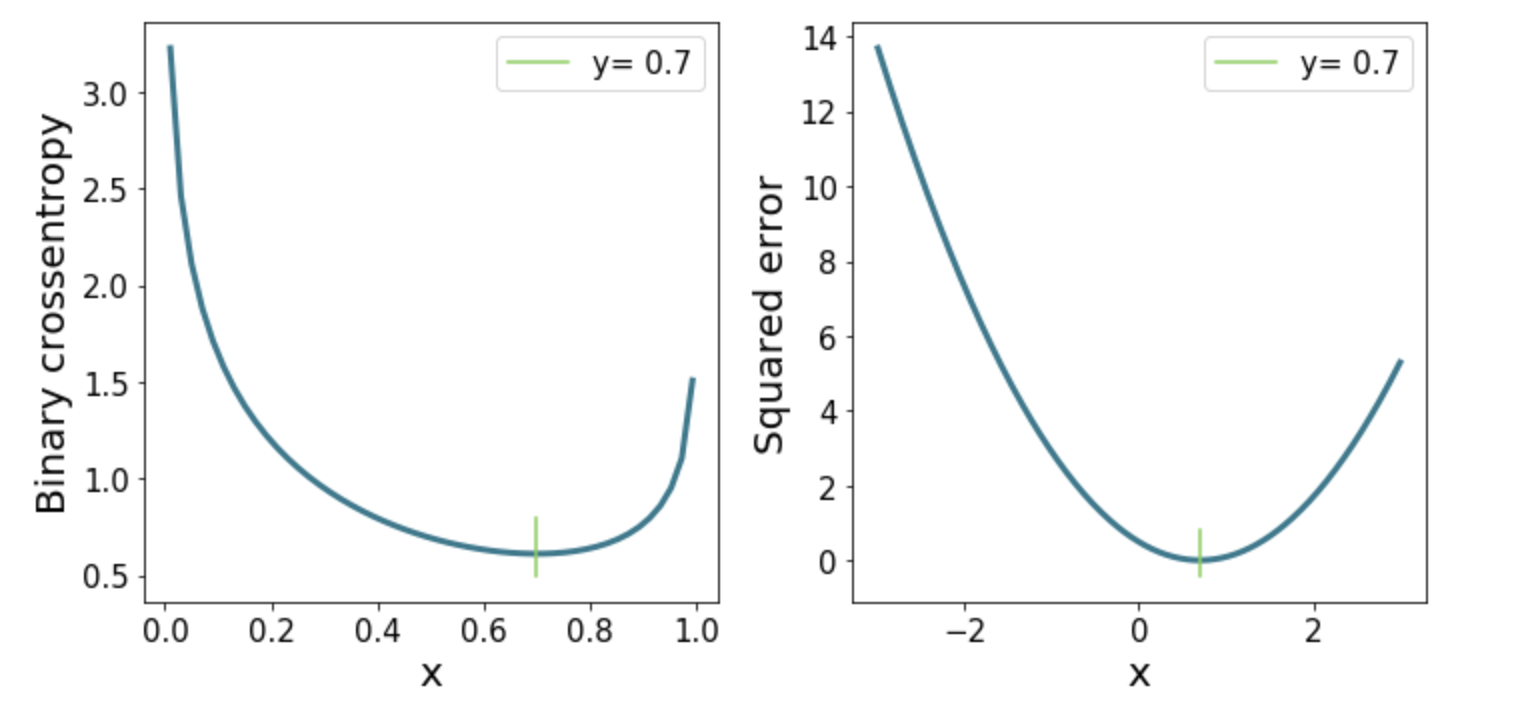
\includegraphics[width=\textwidth]{plots/loss_func_shape.png}
% \caption[Illustrating differences in the shapes of the MSE and BCE-loss]{Illustrating the difference between the function shapes of binary cross-entropy and the mean squared error for the same target value $y=0.7$. We observe that though the two functions have the same minimum the landscape surrounding it is very different. Perhaps most telling is the asymmetry of the cross entropy, implicitly telling the optimizer that values above the targets are measurably worse than those below as measured by the steepness of the gradient. For the AT-TPC data this then implies that predicting higher charge values are worse than predicting lower than the target, and implication that is not physically substantiated}\label{fig:loss_func_shape}
% \end{figure}